\documentclass[twocolumn,10pt]{article}
\usepackage{ragged2e}
\usepackage{csquotes}
\usepackage{amsmath}
\usepackage{array}
\newcolumntype{C}{>$c<$}
\usepackage{mathtools}
%\usepackage{float}
\usepackage{hyperref}
\usepackage{amssymb}
\usepackage{amsthm}
\usepackage{bigints}
\usepackage{esvect}
\usepackage{pgfplots}
\usepackage{xcolor}
\usepackage{tikz}
\usepackage{multicol}
\usepackage{nonfloat}
\usepackage{wrapfig}
\newcommand*\circled[1]{\tikz[baseline=(char.base)]{
            \node[shape=circle,draw,inner sep=2pt] (char) {#1};}}
\usepackage{textcomp}
\RequirePackage{color,graphicx}
\usepackage{graphicx,subcaption}
\usepackage{caption}
\usepackage[paper=letterpaper,margin=0.8in]{geometry}
\newcommand\myeq{\stackrel{\mathclap{\normalfont\mbox{L'H}}}{=}}
\definecolor{amaranth}{rgb}{0.9, 0.17, 0.31}

%custom figure code for multicol
\makeatletter
\newenvironment{tablehere}
  {\def\@captype{table}}
  {}

\newenvironment{figurehere}
  {\def\@captype{figure}}
  {}
\makeatother

\begin{document}

\onecolumn
%---------Put name and information on the top right-----------%
\centering{\huge Project Report: Plant Leaf Health}\\~\\

%\null\hfill\begin{tabular}[t]{l@{}}
\textbf{Hammad Ahmed Sheikh}\\
\textsc{hshammads@csu.fullerton.edu}\\
\textsc{cpsc 483: intro to machine learning}\\
\textsc{fall 2023}\\~\\

\textsc{dr. rong jin}\\
\textsc{california state university, fullerton (CSUF)}\\~\\
%\textsc{November 5, 2023}\\~\\~\\
%\end{tabular}

%---------body of the pitch-----------%
\begin{multicols}{2}
\begin{flushleft}
\justifying

\textit{Abstract} - Precision agriculture has emerged as a pivotal approach in our society to enhance productivity while minimizing resource utilization and is now playing a crucial role in agricultural decision-making processes. The quality and yield of crops are often plagued by diseases, regardless of the season, leading to significant financial loss, not just for farmers but for governments as well. Over the past few recent decades, image processing methodologies have started to be used to detect and classify plant diseases. This study focuses more on personal usage of early disease detection and prevention on personal and private garden. The proposed methodology involves the identification of healthy and unhealthy plant leaves through the application of various techniques, with primary focus on Support Vector Machine (SVM). Clustering-based segmentation is employed via K-means for image segmentation and pre-processing [3] and [7]. Subsequently, classification tasks are undertaken using Support Vector Machine (SVM) models as developed and described by Vegi Shanmukh [4] and [5], and by Sharon Morris [6]. To assess the performance of the proposed methodology, accuracy is evaluated. The comprehensive results demonstrate that the SVM model achieves an accuracy of $81.64\%$ for linear model and \textcolor{red}{NEED TO FILL THIS!!!!!!!!} $\%$ for polynomial model. This research contributes to the advancement of precision agriculture, furthering existing research, by presenting an effective approach for early detection and classification of various plant diseases, facilitating informed decision-making for private citizens, gardeners and farmers.\\
\textit{Keywords} - Precision Agriculture, Plant Disease Detection, Plant Disease Prediction, Machine Learning
	
	\section{Introduction}
	%\begin{flushleft}
	%\justifying
	Gardening is a rejuvenating activity. It is very peaceful and delightful. I enjoy it tremendously. It helps me destress and take a breather from the daily stress of life. My garden consists of flowers, fruits and vegetables. Not only does my garden help me, it also helps the passersby and wild neighborhood animals gain shelter from the sweltering heat. My garden also contributes to mitigating global warming and addressing climate change.\\
	For my garden to do well, it needs to maintained well. There are multiple aspects of maintaining a garden; in-pot soil, in-ground soil, fertilizer, water flow and frequency, sun exposure, soil aeration, pest repellants, supporting plants etc. The biggest hurdle of maintaining a garden is plant health. Each plant is different and requires different amounts of resources, but the same amount of care and attention.\\
	I am fairly new to gardening. Hence, it is difficult for me to be aware of what disease one of my plants have. I can tell when it is sick. However, I am not able to determine the type of care it needs. I have to take a few pictures and show them to gardeners and nursery caretakers to get help. This is not an easy process and requires a lot of effort since there may be people who would not know the disease and its cure - I have to continue asking until I find some who are knowledgeable about my specific problem.\\
	This became an ideal project for me when Dr. Rong Jin at California State University Fullerton [1] assigned Machine Learning class projects in CPSC 483: Intro to Machine Learning.\\
	During my research for a dataset and related research papers I realized that my concerns and problems maintaining my garden are part of a much bigger aspect; agriculture.\\
	Agriculture is a very important part of our lives, especially more so now with the various global conflicts causing shortage in numerous agricultural crops and products, such as wheat, beans and chili. Hence, it is ever-more-so important to maintain the health of the existing crops and ensure that any disease is identified in its early stage and dealt-with immediately.\\
	At present, some farmers request the help of agriculturists to visit their farms and identify the diseases plaguing their crops (same knowledge issue as I have). However, many farmers are not aware of the resource availability of said agriculturists or even that agriculturists can be contacted. Even when farmers are able to contact the agriculturists, it costs a lot of time and money to get an agriculturist to visit their farm. All of this causes the disease the grow in the crops leading to unhealthy cultivation. Hence, there is a need for an automated system for prevention and early disease detection, and providing information the the farmers on how to cure the diseased crops.\\
	 With the development of Machine Learning and Artificial Intelligence, various methods have been introduced for detection of healthy and unhealthy crops, some of which are stated in N. Goyal et al. research paper [8]. The first step to any such model is the detection and existence of a disease. This is still an enormous challenge due to the sheer amount of crops and the variation in the crop images. There are various classification algorithms, such as, but not limited to, Random Forest, K Nearest Neighbors (used by R. Kavitha et al. in basil leaf detection [9]), SVMs [8]. For this project, SVM model is being employed for classifying healthy and unhealthy plants, via feature selection. The dataset being used is the dataset provided by S.S. Chouhan et al [2], which has 12 different plants categorized into healthy and unhealthy plants. Since the data is known, supervised technique can be used for classification - process of categorizing items into clusters on shared characteristics.\\
	Figure \ref{fig:fig1} represents a healthy mango leaf and Figure \ref{fig:fig2} represents an unhealthy mango leaf, obtained from dataset [2].
	%\end{flushleft}
	
	\begin{figurehere}
		\centering
		\includegraphics[width=\linewidth]{healthy_mango.jpg}
		\caption{Healthy Mango Leaf}
		\label{fig:fig1}
	\end{figurehere}
	
	\begin{figurehere}
		\centering
		\includegraphics[width=\linewidth]{diseased_mango.jpg}
		\caption{Diseased Mango Leaf}
		\label{fig:fig2}
	\end{figurehere}
	
	\section{Proposed Methodology}
	The proposed methodology is shown below in Figure \ref{fig:fig3} (Image Acquisition $\rightarrow$ Image Pre-Processing (including Segmentation) $\rightarrow$ Classification).

	\begin{figurehere}
		\centering
		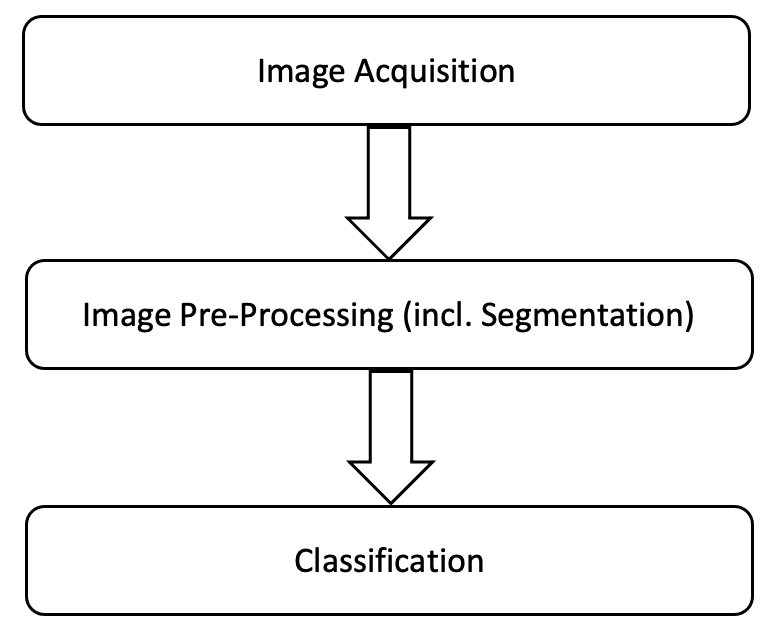
\includegraphics[width=\linewidth]{proposed_methodology2.png}
		\caption{Flow Process of Proposed Methodology}
		\label{fig:fig3}
	\end{figurehere}
	
	\subsection{Image Acquisition}
	The first step in image processing, regardless of whether it is for my specific project of plant leaf health or other projects, is image acquisition. We need to have a dataset that can be used to train the model. My project uses dataset obtained from mendeley repository [2].\\
	Here is the information regarding the dataset from the developers [2]; the images are captured in a closed environment. This acquisition process was completely wi-fi enabled. All the images are captured using a Nikon D5300 camera inbuilt with performance timing for shooting JPEG in single shot mode (seconds/frame, max resolution) = 0.58 and for RAW+JPEG = 0.63. The images were in .jpg format captured with 18-55mm lens with sRGB color representation, 24-bit depth, 2 resolution unit, 1000-ISO, and no flash.
	
	\subsection{Image Pre-Processing (including Segmentation)}
	The original images obtained from the dataset [2] contain a lot of information. We need to reduce the background noise (if not eliminate it), minimize unwanted distortion, and improve focus on the leaf. We also need to decrease the images' size to improve model run time, as processing 7.32 GB of data may not be the fastest, especially on my local personal computer.\\
	Segmentation is a crucial stage in the field of image processing [9 - 11]. Hence, in the pre-processing step, segmentation was encompassed as well. Since we are getting the images ready for model, it was to best to pre-process and segment the images at the same time.\\
	Clustering-based segmentation is employed via K-means for image segmentation and pre-processing [3] and [7].\\
	Initially, I resized the images first and then processed them through the K-means segmentation. Though this process was fast, the images' data quality and value fell drastically. This is because K-means clustering was working with much smaller area of an image after resizing compared with the original image. Hence, it was neither optimal nor efficient.\\
	Therefore, I updated my pre-processing step to run K-means clustering segmentation on every image first and then resize the images. This worked well, and the data quality improved. The overall dataset size decreased to 30 MB post pre-processing. I also created a separate segmented dataset without resizing, in case my computer is able to process a larger sized amount of data. Its size is at 4.53 GB post pre-processing.\\
	Figure \ref{fig:fig4} is the resulting image post pre-processing (including segmentation) for Figure \ref{fig:fig1} and Figure \ref{fig:fig5} is the resulting image post pre-processing (including segmentation) for Figure \ref{fig:fig2}.

	\begin{figurehere}
		\centering
		\includegraphics[width=\linewidth]{healthy_mango_segmented.jpg}
		\caption{Healthy Mango Leaf Segmented}
		\label{fig:fig4}
	\end{figurehere}
	
	\begin{figurehere}
		\centering
		\includegraphics[width=\linewidth]{diseased_mango_segmented.jpg}
		\caption{Diseased Mango Leaf Segmented}
		\label{fig:fig5}
	\end{figurehere}

	
	\subsection{Classification}
	The classification process employs SVM and HOG techniques. SVM is used for classification by transforming the data and identifying optimal boundaries between potential outputs. Moreover, it is useful ins solving both linear and non-linear problems.\\
	
	\section{Experiment Result}
	SVM model by Vegi Shanmukh [4] would not compile on my computer. It ran for quite a while, for both the 30 MB dataset and for the 4.53 GB dataset mentioned in \enquote{Image Pre-Processing (including Segmentation}. Fortunately, my computer was able to compile and build a linear SVM model based on the information provided by Sharon Morris [6], for the 30 MB dataset. The model took 1 hour(s) and 22 minute(s) and 40 second(s) to compile, and achieved an accuracy rate of $81.64\%$.\\
	\textcolor{red}{FILL THIS AFTER MODEL COMPLETION}
	
	\section{Conclusion and Future Work}
	Identifying diseased leaves (and therefore plants) at an early stage assists farmers in preventing significant losses. This enables us to be more efficient in the usage of the limited resources we have available on our planet. In this project, I obtained an existing dataset, pre-processed and segmented it using K-means clustering, and used SVM for classification. In future, the analysis can be done by extending the dataset [2] with more plants and a more diverse set of leaves. The project can also be extended to identify the diseases, as done by Gopal et al [12], where they classified and identified five classes of diseases based on the analysis of basil leaves, including gray mold, fusarium wilt, bacterial leaf spot, and downy mildew. The project can then be extended to propose cures for the diseased plants. This would generate the following life cycle; image acquisition $\rightarrow$ image pre-processing (including segmentation) $\rightarrow$ classification of plant $\rightarrow$ classification of health $\rightarrow$ classification of disease $\rightarrow$ proposed cure for disease.
\end{flushleft}


	
\centering{\huge References}\\~\\
\begin{flushleft}
\begin{enumerate}
	\item Dr. Rong Jin, California State University Fullerton \url{https://www.fullerton.edu/ecs/cs/faculty/}
	\item S. S. Chouhan, U. P. Singh, A. Kaul and S. Jain, \enquote{A Data Repository of Leaf Images: Practice towards Plant Conservation with Plant Pathology}, \textit{2019 4th International Conference on Information Systems and Computer Networks (ISCON)}, Mathura, India, 2019, pp. 700-707, doi: 10.1109/ISCON47742.2019.9036158. \url{https://data.mendeley.com/datasets/hb74ynkjcn/5}
	\item How to implement Image Segmentation in ML, by Emmanuel Kendagor \url{https://cnvrg.io/image-segmentation/}
	\item Image Classification Using Machine Learning-Support Vector Machine(SVM), by Vegi Shanmukh \url{https://rb.gy/8uwxir} %This is the full unshortened URL \url{https://medium.com/analytics-vidhya/image-classification-using-machine-learning-support-vector-machine-svm-dc7a0ec92e01}
	\item GitHub repository for Image Classification Using Machine Learning-Support Vector Machine(SVM), by Vegi Shanmukh \url{https://rb.gy/16m5qz} %This is the full unshortened URL \url{https://github.com/ShanmukhVegi/Image-Classification/tree/main}
	\item Image Classification Using SVM, by Sharon Morris \url{https://rpubs.com/Sharon_1684/454441}
	\item Kumari, C. U., Prasad, S. J., \& Mounika, G. (2019, March), Leaf disease detection: feature extraction with K-means clustering and classification with ANN. In \textit{2019 3rd International Conference on Computing Methodologies and Communication (ICCMC)} (pp. 1095-1098). IEEE.
	\item N. Goyal, S. Kumar and M. Saraswat, \enquote{Detection of Unhealthy citrus leaves using Machine Learning Technique}, \textit{2022 12th International Conference on Cloud Computing, Data Science \& Engineering (Confluence)}, Noida, India, 2022, pp. 591-595, doi: 10.1109/Confluence52989.2022.9734162.
	\item R. Kavitha, M. Kavitha, R. Srinivasan, N. R. Rajalakshmi and R. Dhayanidhi, \enquote{Basil Leaf Diseases Detection using Deep Learning architectures}, \textit{2022 IEEE 19th India Council International Conference (INDICON)}, Kochi, India, 2022, pp. 1-5, doi: 10.1109/INDICON56171.2022.10040158.
	\item Zaitoun, N. M., \& Aqel, M. J. (2015). Survey on Image Segmentation Techniques. Procedia Computer Science, 65 (December), pp. 797-806, doi: 10.1016/j.procs.2015.09.027 \url{https://doi.org/10.1016/j.procs.2015.09.027}
	\item Singh, V., \& Misra, A. K. (2017). Detection of plant leaf diseases using image segmentation and soft computing techniques. Information Processing in Agriculture, 4(1), pp. 41-49, doi: 10.1016/j.inpa.2016.10.005 \url{https://doi.org/10.1016/j.inpa.2016.10.005}
	\item S. S. Kumar and B. K. Raghavendra, \enquote{Diseases Detection of Various Plant Leaf Using Image Processing Techniques: A Review}, \textit{2019 5th International Conference on Advanced Computing \& Communication Systems (ICACCS)}, Coimbatore, India, 2019, pp. 313-316, doi: 10.1109/ICACCS.2019.8728325.
\end{enumerate}
\end{flushleft}
\end{multicols}
\end{document}